\section{Tools}
In this section, we will describe the tools we use and have used to create our system.

\subsection{Arduino Controller}
We had the idea not to only test our code in an application, but also to see live what is happening in our system. From that idea, we decided to create thanks to an Arduino Due controller our traffic lights system. In this controller, we placed LEDs on the boards to imitate the green, orange and red lights of the system. We also added a button for the pedestrians to imitate a real call as we would want to go through a crossroad and another push-button to generate the arrival of a bus in the system. There are also what we call information LEDs that can be lighten up if we arrive in a state that is problematic. This for example means that if all the lights for the cars are green at the same time, there would be a problem in our controller and crashes will thus happen. In this sense, we took some proprieties we modeled for the Verification project and we incorporated them into our embedded system.
\begin{figure}[!ht]\label{fig:arduino}
  \centering
    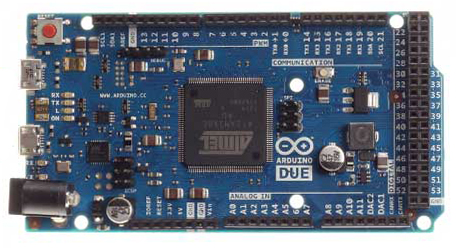
\includegraphics[width=0.5\textwidth]{picture/arduino.jpg}
    \caption{Arduino Due used for the embedded system}
\end{figure} \\
To do so, we wrote the code needed for the good functioning of our system in C.

\subsection{UPPAAL}
Uppaal is a tool box for validation (via graphical simulation) and verification (via automatic model-checking) of real-time systems. The idea is to model a system using timed automata, as defined in Section \ref{sec:automate}, simulate it and then verify properties that we can define on it. Those automata will be synchronized through channels. Because Uppaal is based on timed automata, clocks will be an important thing in this software. Indeed, the time will be handle thanks to those clocks. We will see that it will be possible to test the value of a clock or even to reset it. Also, clocks will progress in the whole system at the same time.
\begin{figure}[h]\label{fig:uppaal}
  \begin{center}
    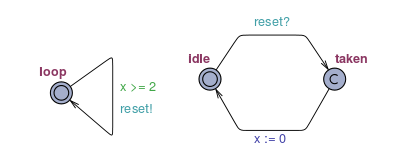
\includegraphics[width=0.8\textwidth]{picture/uppaal.png}
    \caption{Basic example made with UPPAAL}
  \end{center}
\end{figure} \\
 In Figure \ref{fig:uppaal}, two different elements can be seen. On the left part, there is a loop that will, when the clock x is higher or equal to 2, trigger a reset transition. On the right part, we have a system that wait for a reset. When the trigger has been done by the left component, it is send to the right component thanks to the channels between them. If the reset has been done, we transit into the taken state before going back to the Idle state and resetting the x clock to 0. This program then repeat itself.
 
 \subsection{UPPAAL TiGa}
 Tiga is an extension of Uppaal, allowing timed games. The main difference with Uppaal is the possibility of having transitions taken non-deterministically by the environment. Indeed, while in UPPAAL everything is defined by the controller, in TiGa, the environment can also play. Since it's a game between the controller and the environment, we would want to find a winning strategy. In our case, as said in Section \ref{sec:game}, the controller will be the traffic lights while the environment will be the buses and the pedestrians.
 \begin{figure}[h]\label{fig:tiga}
  \begin{center}
    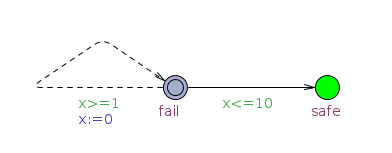
\includegraphics[width=0.8\textwidth]{picture/tiga.png}
    \caption{Basic example made with UPPAAL TiGa}
  \end{center}
\end{figure} \\
In this example, the environment is represented by the cut lines. We start from the fail state and two different states can be reached. Either we go back to the left state because the environment decided to take his transition and to reset the clock x to 0, either to go to the safe state if the controller decided so. 